% !Rnw weave = knitr
\documentclass[12pt,a4paper]{article}\usepackage[]{graphicx}\usepackage[]{xcolor}
% maxwidth is the original width if it is less than linewidth
% otherwise use linewidth (to make sure the graphics do not exceed the margin)
\makeatletter
\def\maxwidth{ %
  \ifdim\Gin@nat@width>\linewidth
    \linewidth
  \else
    \Gin@nat@width
  \fi
}
\makeatother


\newcommand{\hlnum}[1]{\textcolor[rgb]{0.686,0.059,0.569}{#1}}%
\newcommand{\hlsng}[1]{\textcolor[rgb]{0.192,0.494,0.8}{#1}}%
\newcommand{\hlcom}[1]{\textcolor[rgb]{0.678,0.584,0.686}{\textit{#1}}}%
\newcommand{\hlopt}[1]{\textcolor[rgb]{0,0,0}{#1}}%
\newcommand{\hldef}[1]{\textcolor[rgb]{0.345,0.345,0.345}{#1}}%
\newcommand{\hlkwa}[1]{\textcolor[rgb]{0.161,0.373,0.58}{\textbf{#1}}}%
\newcommand{\hlkwb}[1]{\textcolor[rgb]{0.69,0.353,0.396}{#1}}%
\newcommand{\hlkwc}[1]{\textcolor[rgb]{0.333,0.667,0.333}{#1}}%
\newcommand{\hlkwd}[1]{\textcolor[rgb]{0.737,0.353,0.396}{\textbf{#1}}}%
\let\hlipl\hlkwb

\usepackage{framed}
\makeatletter
\newenvironment{kframe}{%
 \def\at@end@of@kframe{}%
 \ifinner\ifhmode%
  \def\at@end@of@kframe{\end{minipage}}%
  \begin{minipage}{\columnwidth}%
 \fi\fi%
 \def\FrameCommand##1{\hskip\@totalleftmargin \hskip-\fboxsep
 \colorbox{shadecolor}{##1}\hskip-\fboxsep
     % There is no \\@totalrightmargin, so:
     \hskip-\linewidth \hskip-\@totalleftmargin \hskip\columnwidth}%
 \MakeFramed {\advance\hsize-\width
   \@totalleftmargin\z@ \linewidth\hsize
   \@setminipage}}%
 {\par\unskip\endMakeFramed%
 \at@end@of@kframe}
\makeatother

\definecolor{shadecolor}{rgb}{.97, .97, .97}
\definecolor{messagecolor}{rgb}{0, 0, 0}
\definecolor{warningcolor}{rgb}{1, 0, 1}
\definecolor{errorcolor}{rgb}{1, 0, 0}
\newenvironment{knitrout}{}{} % an empty environment to be redefined in TeX

\usepackage{alltt}
\usepackage[ansinew]{inputenc}
\usepackage[english]{babel}
\usepackage{amsmath,amsfonts,amssymb}
\usepackage{lmodern}
\usepackage[left=2cm,right=2cm,top=2cm,bottom=2cm]{geometry}
\usepackage{bm}
\usepackage[colorlinks=FALSE]{hyperref}
\usepackage{tabularx}
\usepackage{pdflscape}
\usepackage{pdfpages}
\usepackage{booktabs}
\usepackage{graphicx} %includegraphics
\usepackage{gauss} %für matrix mit Beschriftung

\usepackage{pbox}
\usepackage{longtable}
\usepackage{rotating} %sidewaystable
\usepackage{array}
\usepackage{multirow}
\usepackage{float}
\usepackage{listings} %for Appendix
\usepackage{tikz,pgfplots}
\usetikzlibrary{arrows,shapes.geometric,shapes.arrows,positioning,fit,calc,shapes.symbols,fit}
\pgfplotsset{compat = newest}


\tikzset{%
  highlight/.style={rectangle,rounded corners,draw,thick,inner sep=-3pt}
}
\newcommand{\tikzmark}[2]{\tikz[overlay,remember picture,
  baseline=(#1.base)] \node (#1) {#2};}
%
\newcommand{\Highlight}[1][submatrix]{%
    \tikz[overlay,remember picture]{
    \node[highlight,fit=(left.north west) (right.south east)] (#1) {};}
}

\DeclareMathOperator*{\plim}{plim}
\DeclareMathOperator*{\rel}{rel}
\usepackage{bigdelim} % geschweifte Klammer in table

%\newcolumntype{M}[1]{>{\centering\arraybackslash}m{#1}}

\newcommand{\at}{\makeatletter @\makeatother}
\usepackage{caption}% Für Beschriftung von Grafiken in minipage Umgebung
\usepackage[natbibapa]{apacite}
\usepackage{subfig} %Caption falls mehrere Grafiken in einer Figure Umgebung


\bibliographystyle{apacite}

\DeclareMathOperator*{\var}{\text{var}}
\DeclareMathOperator*{\cor}{\text{cor}}
\DeclareMathOperator*{\cov}{\text{cov}}
\DeclareMathOperator*{\E}{\text{E}}
\DeclareMathOperator*{\argmax}{arg\,max}
\DeclareMathOperator*{\en}{\text{en}}
\DeclareMathOperator*{\ex}{\text{ex}}
\DeclareMathOperator*{\rg}{\text{rg}}

\newcommand\blfootnote[1]{%
  \begingroup
  \renewcommand\thefootnote{}\footnote{#1}%
  \addtocounter{footnote}{-1}%
  \endgroup
}

\newcolumntype{L}[1]{>{\flushleft\arraybackslash}l{#1}}


\newcommand{\pkg}[1]{\textsf{#1}}
\newcommand{\prm}[1]{\texttt{#1}}
\newcommand{\fn}[1]{\texttt{#1}}   % function names
\newcommand{\op}[1]{\texttt{#1}}   % operators / inline code
\IfFileExists{upquote.sty}{\usepackage{upquote}}{}
\begin{document}



\pagenumbering{gobble}


\title{Consistent Partial Least Squares: A cSEM tutorial}
\author{Jason J. Berger, Florian Schuberth}

\date{September 18, 2022}

\newcommand{\Addresses}{{% additional braces for segregating \footnotesize
  \bigskip
  \footnotesize

  Florian Schuberth (corresponding author), \textsc{Faculty of Engineering Technology, University of Twente, P.O. Box 217, 7500 AE Enschede,
The Netherlands}\par\nopagebreak
  \textit{E-mail:} \href{mailto:f.schuberth@utwente.nl}{f.schuberth@utwente.nl},
	\textit{Phone:} +31 53 4897846
}}

\maketitle

\blfootnote{\Addresses}

\newpage

\section*{Abstract}
This tutorial article provides a comprehensive, step-by-step illustration
of consistent partial least squares (PLSc) using the \pkg{cSEM} package in \textsf{R}.
PLSc is a variant of partial least squares path modeling, a composite-based approach to structural equation modeling, that produces consistent parameter estimates for latent variable models.
In particular, PLSc corrects construct correlations for
attenuation using Dijkstra-Henseler's composite reliability coefficient $\varrho_A$.
Building on the employee retention example
introduced by \citet{Cheah2026}, we demonstrate how to install and load
\pkg{cSEM}, specify the model using \pkg{lavaan}-style syntax, estimate the
PLSc-SEM model, evaluate measurement model quality (internal consistency
reliability, convergent validity, and discriminant validity), and assess the
structural model (collinearity, effect sizes, model fit, and path
coefficients with bootstrap inference). We further contrast the PLSc-SEM
results with standard PLS-SEM estimates and discuss practical
considerations for using PLSc-SEM in empirical research.


Keywords: measurement error, bias correction, partial least squares structural equation modeling (PLS-SEM), factor score regression


\newpage

\pagenumbering{arabic}
% \doublespacing

\section*{Introduction}

Structural equation modeling (SEM) is a versatile multivariate analysis framework used in the behavioral, social, medical, and management sciences to study complex relationships between constructs and their relations with observed variables \citep[e.g.,][]{Marcoulides1996,Kline2023}.
To estimate structural equation models, various approaches have been proposed, including maximum-likelihood \citep{Joereskog1970}, weighted least squares \citep{Browne1974}, factor score regression \citep{Skrondal2001,Devlieger2017} and (integrated) generalized structured component analysis \citep{Hwang2004,Hwang2021a}
% Over recent decades, SEM has developed along two conceptually complementary but methodologically distinct
% trajectories: factor-based (covariance-based) SEM (CB-SEM; \citealt{Joreskog1978})
% and composite-based SEM \citep{Wold1974}.

A composite-based estimator to SEM that gained popularity over the last decades in various fields of social sciences \citep{Cook2023}, including marketing \citep{Sarstedt2022a}, information systems research \citep{Benitez2020,Evermann2021}, human resource management \citep{Ringle2020}, and tourism research \citep{Mueller2018}, is partial least squares path modeling \citep[PLS-PM,][]{Wold1982c},also known as partial least squares structural equation modeling \citep[PLS-SEM,][]{Hair2011}.
PLS-PM is a two-step estimation procedure \citep{Schuberth2023d}.
In the first step, construct scores are obtained by the partial least squares algorithm.
Subsequently, these construct scores are used to estimate the model parameters.
Although PLS-PM is computationally efficient, it is known that in its original form to produce inconsistent estimates for models involving latent variables due to attenuation bias \citep[e.g.,][]{Hui1982,Dijkstra1985,Roenkkoe2013,Schuberth2023}.

To address this limitation, consistent partial least squares \citep[PLSc,][]{Dijkstra2013,Dijkstra2014a,Dijkstra2015,Dijkstra2015a} was introduced.
PLSc is based on PLS-PM, but applies a correction for attenuation to obtain consistent estimates of reflective measurement models and path coefficient between latent variables.
Additionally, PLSc has been extended to deal with ordinal variables \citep{Schuberth2018a}, randomly occurring outliers \citep{Schamberger2020} and multicollinearity issues \citep{Jung2018}.

To apply PLS-PM and PLSc, various implementations have been developed \citep{Venturini2023}.
They can be distinguished into: (i) proprietary software and (ii) open-source software.
Proprietary software %is characterized
% Examples of closed-source proprietary software
for conducting PLS-PM and PLSc includes SmartPLS \citep{Ringle2024}, WarpPLS \citep{Kock2025} and ADANCO \citep{adanco}.
On the other hand, open-source software alternatives include implementations in the statistical programming environment R \citep{R} such as matrixpls \citep{Roenkkoe2022a}, SEMinR \citep{seminr}, cSEM \citep{csem} and plspm \citep{Sanchez2025}.
Similarly, it includes implementations in python \citep{python3} such as plspm \citep{Humble2024}.
While proprietary software such as SmartPLS often shows high ease of use \citep{Cheah2024}, they conflict with the open science principles \citep{UNESCO}.
For example, their codebase is not openly accessible of transparency \citep{Morin2012a}, reproducibility \citep{Ince2012}, and accessibility/inclusiveness \citep{}.
Open-source software overcomes these limitations \citep{Barba2022}.
Therefore, this tutorial presents the R package cSEM as a full-fledged open-source alternative to SmartPLS to apply PLS-PM and PLSc.


% of open science because they cost money and thus complicate their use for researchers working at institutions with less resources.
% Similarly, the source code of proprietary software is closed and thus not  open, which turns the software into nontransparent black boxes that hinder the reproducibility of results \citep{Ince2012,Morin2012a},
% In contrast, the source code of open-source software is open \citep{Barba2022} and thus overcomes these limitations as it is free of charge and the codebase is openly available, thus lowering barriers for collaboration.
% Therefore, this tutorial presents cSEM as a full-fledged open-source alternative to SmartPLS  to apply PLS-PM and PLSc.

\citet{Barba2022}

\citep{Chuah2021}

The remainder of the tutorial is structured as follows.
Section
Section
Section


% \citet{Cheah2026} recently provided a comprehensive SmartPLS~4 tutorial for PLSc-SEM analysis. While SmartPLS offers a user-friendly graphical interface, many researchers---particularly those in quantitative methodology, psychometrics, and data science---prefer script-based, open-source tools for their reproducibility, flexibility, and transparency. The \pkg{cSEM} package \citep{Rademaker2020} for R provides a comprehensive, open-source implementation of composite-based SEM methods, including PLSc-SEM, within a unified and well-documented framework.


% Although \textsf{SmartPLS} is the dominant commercial software for PLSc-SEM
% \citep{Cheah2026}, the \pkg{cSEM} package for \textsf{R}
% \citep{Rademaker2020} offers a powerful, freely available, open-source
% alternative. The \pkg{cSEM} package implements PLSc automatically whenever
% any construct in the model is specified as a common factor using the
% \op{=\textasciitilde} operator, making the transition from PLS-SEM to
% PLSc-SEM seamless for \textsf{R} users.

% This tutorial provides a complete, reproducible walkthrough of PLSc-SEM
% estimation using \pkg{cSEM}, mirroring the structure of \citet{Cheah2026}.
% We use the same employee retention dataset \citep{HairBlack2019} to ensure
% direct comparability of results. The tutorial covers package installation,
% model specification, estimation, measurement model evaluation, and structural
% model assessment, concluding with a brief comparison of PLSc-SEM and standard
% PLS-SEM estimates.


\section{cSEM R package Illustration}
\subsection{First steps in \textsf{R}}
This section illustrates how to apply PLSc using the \pkg{cSEM} package, starting from the very first steps.
It assumes no prior experience with \textsf{R};
readers already familiar with \textsf{R} and \textsf{RStudio} may skip directly to Section~\ref{sec:model-data}.

To use the \pkg{cSEM} package, users first need to install \textsf{R} and an integrated development environment (IDE) such as \textsf{RStudio}.
For the installation, we refer to the official guides for \textsf{R} (\url{https://cran.r-project.org}) and \textsf{RStudio} (\url{https://posit.co/download/rstudio-desktop}).

When \textsf{RStudio} is opened for the first time, it displays four panes (Figure~\ref{fig:rstudio}).
The two most important ones are the \emph{script editor} (upper left), where code is written and saved, and the \emph{Console} (lower left), where the code is executed and results are printed.
The \emph{Environment} pane (upper right) lists the objects currently loaded into memory, and the fourth pane (lower right) provides access to files, plots, and help pages.

Although code can be typed directly into the console, it is good practice to work in a script, since a script can be saved, shared, and re-run, which is essential for reproducible analyses.
To create a new script, click \textsf{File~$\rightarrow$ New File~$\rightarrow$ R Script}.
The typical workflow is to write code in the editor and run the selected line(s) with \texttt{Ctrl~+~Enter}.
Any line beginning with \texttt{\#} is treated as a comment: it documents what the code does and is ignored when the code runs.

\begin{knitrout}\small
\definecolor{shadecolor}{rgb}{0.973, 0.973, 0.973}\color{fgcolor}\begin{kframe}
\begin{alltt}
\hlcom{# This is a comment and is not executed.}
\hlnum{1} \hlopt{+} \hlnum{1}   \hlcom{# Code is executed; the result is printed in the Console.}
\end{alltt}
\end{kframe}
\end{knitrout}

Before \pkg{cSEM} can be used, it must be installed. The \pkg{cSEM} package is available on CRAN, so the most recent stable version can be installed with:
\begin{knitrout}\small
\definecolor{shadecolor}{rgb}{0.973, 0.973, 0.973}\color{fgcolor}\begin{kframe}
\begin{alltt}
\hlkwd{install.packages}\hldef{(}\hlsng{"cSEM"}\hldef{)}
\end{alltt}
\end{kframe}
\end{knitrout}
Installation only needs to be done once per machine (rerun this line to update the package later).
Moreover, development versions can be installed from GitHub: \url{https://github.com/FloSchuberth/cSEM}.
After installation, the package must be loaded at the start of every new \textsf{R} session before its functions become available:
\begin{knitrout}\small
\definecolor{shadecolor}{rgb}{0.973, 0.973, 0.973}\color{fgcolor}\begin{kframe}
\begin{alltt}
\hlkwd{library}\hldef{(cSEM)}
\end{alltt}
\end{kframe}
\end{knitrout}
With \pkg{cSEM} installed and loaded, we can now import the data and specify the model, as described in the following sections.

\begin{figure}[htbp]
\centering
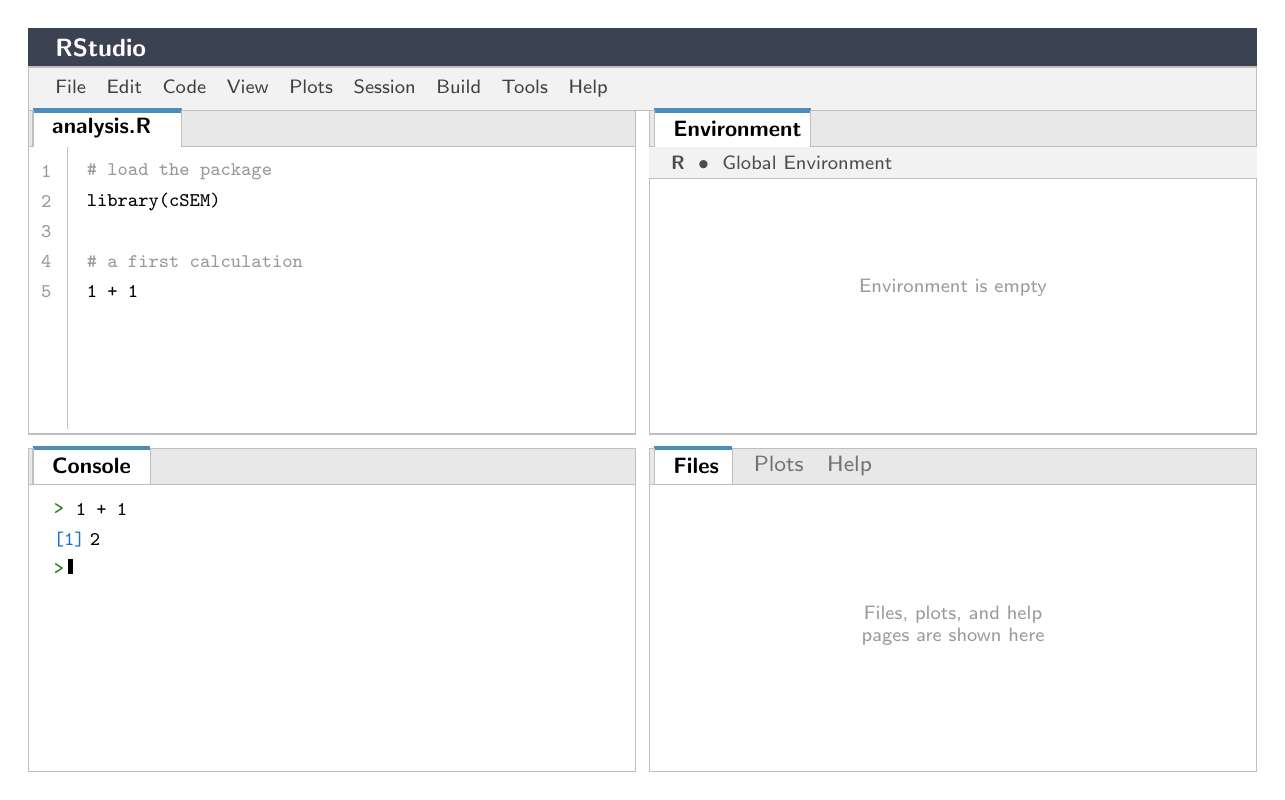
\begin{tikzpicture}[font=\sffamily]
% ---- colors ----
\definecolor{rsbar}{HTML}{3B4252}      % dark toolbar
\definecolor{rsmenu}{HTML}{F2F2F2}     % menu bar
\definecolor{rstab}{HTML}{E8E8E8}      % tab strip
\definecolor{rspane}{HTML}{FFFFFF}     % pane body
\definecolor{rsborder}{HTML}{BFBFBF}   % borders
\definecolor{rsaccent}{HTML}{4C8DBE}   % active tab accent (blue)
\definecolor{rsprompt}{HTML}{1A7D1A}   % console green prompt
\definecolor{rscomment}{HTML}{9A9A9A}  % comment grey
\definecolor{rsnum}{HTML}{1873CC}      % numeric output blue

% geometry
\def\W{15.6}    % total width
\def\H{8.4}     % total height (panes)
\def\gap{0.18}  % gap between panes
\def\tabh{0.46} % tab strip height

% pane sizes
\pgfmathsetmacro{\paneW}{(\W-\gap)/2}
\pgfmathsetmacro{\paneH}{(\H-\gap)/2}

% positions
\def\lx{0}
\pgfmathsetmacro{\rx}{\paneW+\gap}
\def\by{0}
\pgfmathsetmacro{\ty}{\paneH+\gap}

% ===================== title + menu bar =====================
\fill[rsbar]  (0,\H+0.55) rectangle (\W,\H+1.05);
\node[white,font=\sffamily\small\bfseries,anchor=west] at (0.22,\H+0.80) {RStudio};
\fill[rsmenu] (0,\H) rectangle (\W,\H+0.55);
\draw[rsborder] (0,\H) rectangle (\W,\H+0.55);
\node[anchor=west,font=\sffamily\scriptsize,text=black!75] at (0.22,\H+0.275)
  {File\quad Edit\quad Code\quad View\quad Plots\quad Session\quad Build\quad Tools\quad Help};

% ===================== pane frame macro =====================
% #1 x, #2 y (lower-left)
\newcommand{\paneframe}[2]{
  \fill[rspane] (#1,#2) rectangle (#1+\paneW,#2+\paneH);
  \fill[rstab]  (#1,#2+\paneH-\tabh) rectangle (#1+\paneW,#2+\paneH);
  \draw[rsborder] (#1,#2) rectangle (#1+\paneW,#2+\paneH);
  \draw[rsborder] (#1,#2+\paneH-\tabh) -- (#1+\paneW,#2+\paneH-\tabh);
}
% active tab highlight: #1 x #2 y(pane LL) #3 tab-left #4 tab-right
\newcommand{\activetab}[4]{
  \fill[rspane] (#1+#3,#2+\paneH-\tabh) rectangle (#1+#4,#2+\paneH);
  \draw[rsaccent,line width=1.6pt] (#1+#3,#2+\paneH) -- (#1+#4,#2+\paneH);
  \draw[rsborder] (#1+#3,#2+\paneH-\tabh) -- (#1+#3,#2+\paneH);
  \draw[rsborder] (#1+#4,#2+\paneH-\tabh) -- (#1+#4,#2+\paneH);
}

% ---- four pane frames ----
\paneframe{\lx}{\ty}   % top-left  Source
\paneframe{\lx}{\by}   % bottom-left Console
\paneframe{\rx}{\ty}   % top-right Environment
\paneframe{\rx}{\by}   % bottom-right Files

% ---- active tabs ----
\activetab{\lx}{\ty}{0.06}{1.95}   % analysis.R
\activetab{\lx}{\by}{0.06}{1.55}   % Console
\activetab{\rx}{\ty}{0.06}{2.05}   % Environment
\activetab{\rx}{\by}{0.06}{1.05}   % Files

% ---- tab labels ----
\node[anchor=west,font=\sffamily\footnotesize\bfseries] at (\lx+0.18,\ty+\paneH-\tabh/2) {analysis.R};
\node[anchor=west,font=\sffamily\footnotesize\bfseries] at (\lx+0.18,\by+\paneH-\tabh/2) {Console};
\node[anchor=west,font=\sffamily\footnotesize\bfseries] at (\rx+0.18,\ty+\paneH-\tabh/2) {Environment};
\node[anchor=west,font=\sffamily\footnotesize\bfseries] at (\rx+0.18,\by+\paneH-\tabh/2) {Files};
\node[anchor=west,font=\sffamily\footnotesize,text=black!55] at (\rx+1.20,\by+\paneH-\tabh/2) {Plots\quad Help};

% ====== Script editor (top-left) ======
\begin{scope}[shift={(\lx,\ty)},font=\ttfamily\scriptsize]
  \def\cy{\paneH-\tabh-0.32}     % first code line y
  \def\dy{0.38}                  % line step
  \draw[rsborder] (0.50,\paneH-\tabh) -- (0.50,0.06);   % gutter rule
  \foreach \n in {1,...,5}{
    \pgfmathsetmacro{\yy}{\cy-\dy*(\n-1)}
    \node[anchor=east,rscomment] at (0.42,\yy) {\n};
  }
  \node[anchor=west,rscomment] at (0.62,\cy)        {\# load the package};
  \node[anchor=west,black]     at (0.62,\cy-\dy)    {library(cSEM)};
  \node[anchor=west,rscomment] at (0.62,\cy-3*\dy)  {\# a first calculation};
  \node[anchor=west,black]     at (0.62,\cy-4*\dy)  {1 + 1};
\end{scope}

% ====== Console (bottom-left) ======
\begin{scope}[shift={(\lx,\by)},font=\ttfamily\scriptsize]
  \def\cy{\paneH-\tabh-0.32}
  \def\dy{0.38}
  \node[anchor=west,rsprompt] at (0.20,\cy)        {>};
  \node[anchor=west,black]    at (0.48,\cy)        {1 + 1};
  \node[anchor=west,rsnum]    at (0.20,\cy-\dy)    {[1]};
  \node[anchor=west,black]    at (0.66,\cy-\dy)    {2};
  \node[anchor=west,rsprompt] at (0.20,\cy-2*\dy)  {>};
  \fill[black] (0.50,\cy-2*\dy-0.06) rectangle (0.57,\cy-2*\dy+0.13); % cursor
\end{scope}

% ====== Environment (top-right) ======
\begin{scope}[shift={(\rx,\ty)},font=\sffamily\scriptsize]
  % sub-header bar
  \fill[rsmenu] (0,\paneH-\tabh-0.40) rectangle (\paneW,\paneH-\tabh);
  \draw[rsborder] (0,\paneH-\tabh-0.40) -- (\paneW,\paneH-\tabh-0.40);
  \node[anchor=west,font=\sffamily\scriptsize,text=black!70]
    at (0.15,\paneH-\tabh-0.20) {\textbf{R} $\;\bullet\;$ Global Environment};
  \node[anchor=center,rscomment] at (\paneW/2,\paneH/2-0.2) {Environment is empty};
\end{scope}

% ====== Files / Plots / Help (bottom-right) ======
\begin{scope}[shift={(\rx,\by)},font=\sffamily\scriptsize]
  \node[anchor=center,rscomment,align=center] at (\paneW/2,\paneH/2-0.2)
    {Files, plots, and help\\pages are shown here};
\end{scope}

\end{tikzpicture}
\caption{The four panes of the \textsf{RStudio} interface: the script editor
(upper left), the \emph{Console} (lower left), the \emph{Environment} pane
(upper right), and the files/plots/help pane (lower right).}
\label{fig:rstudio}
\end{figure}

\subsection{Model and Data}
\label{sec:model-data}
The \pkg{cSEM} package \citep{csem} offers a variety of composite-based approaches to SEM including PLS-PM and PLSc.
To illustrate the application of PLSc using cSEM, we use the data and model used in \citet{Cheah2026} to demonstrate SmartPLS.
Similarly, we compare the results to those of the maximum-likelihood estimation as implemented in the R package lavaan \citep{Rosseel2012,Rosseel2025}.

Following \citet{Cheah2026}, our illustration draws on the employee retention model introduced by \citet[Chapter~13]{Hair2019c}.
The model explains the effects of organizational commitment~(OC) and job satisfaction~(JS) on employees' staying intentions~(SI), with work environment perceptions~(EP) and attitudes toward coworkers~(AC) as exogenous antecedent constructs.
Five constructs are reflectively measured by a total of 21 indicators.
A detailed description of the indicators can be found in \citet{Cheah2026}.
The model is presented in Figure \ref{fig:retentionmodel}.

\begin{figure}
    \centering
    
\includegraphics[width=0.7\linewidth]{"plots/retention_model_preview.png"}
    \caption{Employee Retention Model}
    \label{fig:retentionmodel}
\end{figure}

The central function is \fn{csem()}, which accepts a model specification in \pkg{lavaan}-style syntax and a dataset, and returns an object containing all estimation results.
Key arguments include:
\begin{description}
  \item[\prm{.data}] A data frame or matrix containing the observed indicator variables.
  \item[\prm{.model}] A model string written in \pkg{lavaan} syntax, with \texttt{=\textasciitilde} for measurement relations and \texttt{\textasciitilde} for structural (regression) relations.
  \item[\prm{.approach\_weights}] The weighting scheme for computing composite scores. Set to \texttt{"PLS-PM"} for PLS-based estimation (the default).
  \item[\prm{.disattenuate}] Logical. When set to \texttt{TRUE}, \pkg{cSEM} applies the PLSc correction for attenuation, yielding consistent estimates under the common factor model. This is the key switch that distinguishes PLSc-SEM from standard PLS-SEM.
  \item[\prm{.PLS\_weight\_scheme\_inner}] The inner weighting scheme; options include \texttt{"path"} (default), \texttt{"centroid"}, and \texttt{"factorial"}.
\end{description}

When using their own data, users must ensure it is stored as a data frame or a matrix before passing it to \pkg{cSEM} functions; if necessary, the data can be converted with \fn{as.data.frame()} or \fn{as.matrix()}.

Additional post estimation functions include \fn{assess()} for measurement and structural model quality criteria, \fn{summarize()} for a comprehensive results summary, \fn{infer()} for bootstrap-based inference, \fn{testOMF()} for the overall model fit test, and \fn{predict()} for out-of-sample prediction.


\subsection{Model specification}
In \pkg{cSEM}, models are specified using \pkg{lavaan} model syntax.
In particular, the \texttt{=~} and the \texttt{<~} operators are used to define the relations between the constructs and their indicators.
Specifically, the \texttt{=~} operator is used to specify reflective measurement models, while the \texttt{<~} is used to specify composite models \citep[see][for an explanation of reflective and composite models]{}.
In addition, the \texttt{~} operator is used to specify the relations among constructs.
In case, an observed variable should be directly accounted for in the structural model, it must be specified as a single indicator construct, as common in PLS-PM \citep{}.
The \pkg{cSEM} specification of the retention model illustrated in Figure \ref{fig:retentionmodel} is as follows:

\begin{knitrout}\small
\definecolor{shadecolor}{rgb}{0.973, 0.973, 0.973}\color{fgcolor}\begin{kframe}
\begin{alltt}
\hldef{model} \hlkwb{<-} \hlsng{"
  # Measurement model
  AC =~ AC1 + AC2 + AC3 + AC4
  EP =~ EP1 + EP2 + EP3 + EP4
  JS =~ JS1 + JS2 + JS3 + JS4 + JS5
  OC =~ OC1 + OC2 + OC3 + OC4
  SI =~ SI1 + SI2 + SI3 + SI4

  # Structural model
  JS ~ EP + AC
  OC ~ EP + AC + JS
  SI ~ JS + OC
"}
\end{alltt}
\end{kframe}
\end{knitrout}



\subsection{PLSc-SEM Estimation}
The workhorse of the \pkg{cSEM} package is the csem function.
The minimal input required for the csem fucntion is a dataset and a model.
In addition, the csem function shows various arguments that can be used to adjust the PLS algorithm.
These arguments include

To ultimately estimate the model using PLSc-SEM, we call \fn{csem()} with \prm{.disattenuate~=~TRUE}. This single argument activates the consistent correction that distinguishes PLSc-SEM from standard PLS-SEM:

\begin{knitrout}\small
\definecolor{shadecolor}{rgb}{0.973, 0.973, 0.973}\color{fgcolor}\begin{kframe}
\begin{alltt}
\hlcom{# PLSc-SEM estimation}
\hldef{res_plsc} \hlkwb{<-} \hlkwd{csem}\hldef{(}
  \hlkwc{.data}                    \hldef{= hbat_sub,}
  \hlkwc{.model}                   \hldef{= model,}
  \hlkwc{.approach_weights}        \hldef{=} \hlsng{"PLS-PM"}\hldef{,}
  \hlkwc{.disattenuate}            \hldef{=} \hlnum{TRUE}\hldef{,}
  \hlkwc{.PLS_weight_scheme_inner} \hldef{=} \hlsng{"path"}
\hldef{)}

\hlcom{# Verify convergence}
\hlkwd{verify}\hldef{(res_plsc)}
\end{alltt}
\end{kframe}
\end{knitrout}

The \fn{verify()} function checks whether the PLS algorithm converged, whether all construct reliability estimates~($\rho_\text{A}$) are positive (a necessary condition for the PLSc correction), and whether the model-implied indicator correlation matrix is admissible. If all checks pass, the estimation can be considered successful.

To obtain a comprehensive overview of all results, including loadings, path coefficients, reliability measures, and $R^2$ values, use:

\begin{knitrout}\small
\definecolor{shadecolor}{rgb}{0.973, 0.973, 0.973}\color{fgcolor}\begin{kframe}
\begin{alltt}
\hlcom{# Full results summary}
\hldef{summary_res} \hlkwb{<-} \hlkwd{summarize}\hldef{(res_plsc)}
\hlkwd{print}\hldef{(summary_res)}

\hlcom{# For a more compact overview}
\hldef{summary_res}\hlopt{$}\hldef{Estimates}\hlopt{$}\hldef{Loading_estimates}
\hldef{summary_res}\hlopt{$}\hldef{Estimates}\hlopt{$}\hldef{Path_estimates}
\end{alltt}
\end{kframe}
\end{knitrout}

For comparison, standard PLS-SEM (without the consistency correction) can be obtained by setting \prm{.disattenuate~=~FALSE}:

\begin{knitrout}\small
\definecolor{shadecolor}{rgb}{0.973, 0.973, 0.973}\color{fgcolor}\begin{kframe}
\begin{alltt}
\hlcom{# Standard PLS-SEM (without correction)}
\hldef{res_pls} \hlkwb{<-} \hlkwd{csem}\hldef{(}
  \hlkwc{.data}             \hldef{= hbat_sub,}
  \hlkwc{.model}            \hldef{= model,}
  \hlkwc{.approach_weights} \hldef{=} \hlsng{"PLS-PM"}\hldef{,}
  \hlkwc{.disattenuate}     \hldef{=} \hlnum{FALSE}
\hldef{)}
\end{alltt}
\end{kframe}
\end{knitrout}

% ── 3.4 Measurement Model Assessment ─────────────────────────────────
\subsection{Measurement Model Assessment}

Following the guidelines described in \citet[Chapter~4]{Hair2026primer} and \citet{Sarstedt2025}, we assess the reflective measurement model in terms of internal consistency reliability, convergent validity, and discriminant validity. The \fn{assess()} function in \pkg{cSEM} provides all relevant quality criteria:

\begin{knitrout}\small
\definecolor{shadecolor}{rgb}{0.973, 0.973, 0.973}\color{fgcolor}\begin{kframe}
\begin{alltt}
\hlcom{# Compute all quality criteria}
\hldef{quality} \hlkwb{<-} \hlkwd{assess}\hldef{(res_plsc)}

\hlcom{# Internal consistency reliability}
\hldef{quality}\hlopt{$}\hldef{Cronbachs_alpha}      \hlcom{# Cronbach's alpha}
\hldef{quality}\hlopt{$}\hldef{RhoA}                 \hlcom{# Dijkstra-Henseler rho_A}
\hldef{quality}\hlopt{$}\hldef{RhoC}                 \hlcom{# Composite reliability (Joreskog rho_C)}

\hlcom{# Convergent validity}
\hldef{quality}\hlopt{$}\hldef{AVE}                  \hlcom{# Average variance extracted}

\hlcom{# Indicator loadings}
\hldef{summary_res}\hlopt{$}\hldef{Estimates}\hlopt{$}\hldef{Loading_estimates}
\end{alltt}
\end{kframe}
\end{knitrout}

% ── Table 1 ──────────────────────────────────────────────────────────
\begin{table}[htbp]
\centering
\caption{Reflective measurement model assessment results (PLSc-SEM via \pkg{cSEM}).}
\label{tab:measurement}
\small
\begin{tabular}{llccccc}
\toprule
Construct & Item & Outer loading & Cronbach's $\alpha$ & $\rho_\text{A}$ & $\rho_\text{C}$ & AVE \\
\midrule
AC & AC1 & 0.770 & 0.894 & 0.911 & 0.926 & 0.679 \\
   & AC2 & 0.677 & & & & \\
   & AC3 & 0.823 & & & & \\
   & AC4 & 0.993 & & & & \\[3pt]
EP & EP1 & 0.631 & 0.857 & 0.869 & 0.903 & 0.605 \\
   & EP2 & 0.875 & & & & \\
   & EP3 & 0.763 & & & & \\
   & EP4 & 0.821 & & & & \\[3pt]
JS & JS1 & 0.618 & 0.844 & 0.856 & 0.888 & 0.518 \\
   & JS2 & 0.696 & & & & \\
   & JS3 & 0.715 & & & & \\
   & JS4 & 0.628 & & & & \\
   & JS5 & 0.903 & & & & \\[3pt]
OC & OC1 & 0.427 & 0.832 & 0.887 & 0.886 & 0.573 \\
   & OC2 & 0.958 & & & & \\
   & OC3 & 0.682 & & & & \\
   & OC4 & 0.852 & & & & \\[3pt]
SI & SI1 & 0.817 & 0.889 & 0.899 & 0.923 & 0.672 \\
   & SI2 & 0.870 & & & & \\
   & SI3 & 0.677 & & & & \\
   & SI4 & 0.897 & & & & \\
\bottomrule
\end{tabular}

\smallskip
\footnotesize\textit{Note.} AC = attitudes toward coworkers; EP = environment perceptions; JS = job satisfaction; OC = organizational commitment; SI = staying intentions. Results replicate those in \citet[Table~1]{Cheah2026}.
\end{table}

The results in Table~\ref{tab:measurement} indicate that all constructs meet the commonly accepted thresholds. All Cronbach's~$\alpha$ and $\rho_\text{A}$ values exceed 0.70, and all AVE values exceed 0.50, supporting internal consistency reliability and convergent validity. While some outer loadings (e.g., OC1~=~0.427) fall below the recommended threshold of 0.708, these indicators are retained because the corresponding constructs exhibit adequate reliability and AVE, and their retention preserves content validity \citep{Hair2026primer}.

% ── 3.4.1 HTMT ────────────────────────────────────────────────────────
\subsubsection{Discriminant Validity: The HTMT Criterion}

Discriminant validity is assessed using the heterotrait-monotrait ratio of correlations \citep[HTMT;][]{Henseler2015}. In \pkg{cSEM}, HTMT values are available via \fn{assess()}:

\begin{knitrout}\small
\definecolor{shadecolor}{rgb}{0.973, 0.973, 0.973}\color{fgcolor}\begin{kframe}
\begin{alltt}
\hlcom{# HTMT values}
\hldef{quality}\hlopt{$}\hldef{HTMT}

\hlcom{# Bootstrap confidence intervals for HTMT}
\hldef{res_plsc_boot} \hlkwb{<-} \hlkwd{csem}\hldef{(}
  \hlkwc{.data}             \hldef{= hbat_sub,}
  \hlkwc{.model}            \hldef{= model,}
  \hlkwc{.approach_weights} \hldef{=} \hlsng{"PLS-PM"}\hldef{,}
  \hlkwc{.disattenuate}     \hldef{=} \hlnum{TRUE}\hldef{,}
  \hlkwc{.resample_method}  \hldef{=} \hlsng{"bootstrap"}\hldef{,}
  \hlkwc{.R}                \hldef{=} \hlnum{10000}\hldef{,}
  \hlkwc{.seed}             \hldef{=} \hlnum{42}
\hldef{)}

\hlcom{# Extract HTMT inference}
\hldef{htmt_infer} \hlkwb{<-} \hlkwd{infer}\hldef{(res_plsc_boot)}
\hlcom{# The infer() output includes CIs for all quality criteria}
\hlcom{# including HTMT values}
\end{alltt}
\end{kframe}
\end{knitrout}

% ── Table 2 ──────────────────────────────────────────────────────────
\begin{table}[htbp]
\centering
\caption{HTMT criterion results.}
\label{tab:htmt}
\small
\begin{tabular}{lcccc}
\toprule
Construct & AC & EP & JS & OC \\
\midrule
EP & 0.257 {[0.163; 0.347]} & & & \\
JS & 0.066 {[0.032; 0.075]} & 0.244 {[0.164; 0.326]} & & \\
OC & 0.275 {[0.195; 0.355]} & 0.495 {[0.405; 0.580]} & 0.209 {[0.118; 0.297]} & \\
SI & 0.310 {[0.222; 0.395]} & 0.569 {[0.471; 0.656]} & 0.232 {[0.154; 0.313]} & 0.501 {[0.410; 0.586]} \\
\bottomrule
\end{tabular}

\smallskip
\footnotesize\textit{Note.} Values in brackets: 90\% percentile bootstrap confidence intervals (10,000 subsamples).
\end{table}

The HTMT results in Table~\ref{tab:htmt} confirm discriminant validity: none of the upper bounds of the 90\% bootstrap confidence intervals exceed the conservative threshold of 0.85 \citep{Henseler2015, Franke2019}. These findings are identical to those reported by \citet[Table~2]{Cheah2026}, confirming that the \pkg{cSEM} results replicate the SmartPLS output.

% ── 3.5 Structural Model Assessment ──────────────────────────────────
\subsection{Structural Model Assessment}

\subsubsection{Collinearity Assessment}

Before interpreting the structural model, we check for collinearity among predictor constructs by examining variance inflation factors (VIF). In \pkg{cSEM}, VIF values are available through the \fn{assess()} function:

\begin{knitrout}\small
\definecolor{shadecolor}{rgb}{0.973, 0.973, 0.973}\color{fgcolor}\begin{kframe}
\begin{alltt}
\hlcom{# VIF values for structural model}
\hldef{quality}\hlopt{$}\hldef{VIF}
\end{alltt}
\end{kframe}
\end{knitrout}

All VIF values should be below the critical threshold of three \citep{Hair2026primer}, indicating that multicollinearity is not a concern.

\subsubsection{Path Coefficients and Bootstrap Inference}

To evaluate the statistical significance of the structural relationships, we rely on bootstrap confidence intervals. The bootstrap estimation was already conducted above. Path coefficients and their confidence intervals are extracted as follows:

\begin{knitrout}\small
\definecolor{shadecolor}{rgb}{0.973, 0.973, 0.973}\color{fgcolor}\begin{kframe}
\begin{alltt}
\hlcom{# Extract path coefficient estimates}
\hlkwd{summarize}\hldef{(res_plsc)}\hlopt{$}\hldef{Estimates}\hlopt{$}\hldef{Path_estimates}

\hlcom{# Bootstrap inference for path coefficients}
\hldef{boot_infer} \hlkwb{<-} \hlkwd{infer}\hldef{(res_plsc_boot)}

\hlcom{# Percentile bootstrap confidence intervals (95%)}
\hldef{boot_infer}\hlopt{$}\hldef{Path_estimates}\hlopt{$}\hldef{CI_percentile}
\end{alltt}
\end{kframe}
\end{knitrout}

% ── Table 3 ──────────────────────────────────────────────────────────
\begin{table}[htbp]
\centering
\caption{Structural model assessment results.}
\label{tab:structural}
\small
\begin{tabular}{lccccccc}
\toprule
Relationship & Path coeff. & SD & $t$ value & $p$ value & 95\% CI & VIF & $f^2$ \\
\midrule
AC $\to$ JS & $-$0.002 & 0.058 & 0.043 & .966 & [$-$0.119; 0.106] & 1.055 & 0.000 \\
AC $\to$ OC &    0.172 & 0.048 & 3.619 & .000 & [0.078; 0.264]    & 1.055 & 0.039 \\
EP $\to$ JS &    0.245 & 0.053 & 4.641 & .000 & [0.136; 0.343]    & 1.055 & 0.060 \\
EP $\to$ OC &    0.430 & 0.059 & 7.272 & .000 & [0.309; 0.540]    & 1.101 & 0.227 \\
JS $\to$ OC &    0.095 & 0.052 & 1.820 & .069 & [$-$0.011; 0.194] & 1.047 & 0.012 \\
JS $\to$ SI &    0.132 & 0.046 & 2.833 & .005 & [0.043; 0.225]    & 1.035 & 0.023 \\
OC $\to$ SI &    0.490 & 0.051 & 9.520 & .000 & [0.386; 0.587]    & 1.035 & 0.321 \\
\bottomrule
\end{tabular}

\smallskip
\footnotesize\textit{Note.} CI = 95\% percentile bootstrap confidence interval (10,000 subsamples). Results replicate \citet[Table~3]{Cheah2026}.
\end{table}

The structural model results in Table~\ref{tab:structural} are consistent with those reported by \citet[Table~3]{Cheah2026}. Based on the 95\% percentile bootstrap confidence intervals, all structural relationships are statistically significant except for the paths from AC to JS ($\beta = -0.002$, $p = .966$) and from JS to OC ($\beta = 0.095$, $p = .069$). Environment perceptions~(EP) exert the strongest positive effect on organizational commitment ($\beta = 0.430$), which in turn is the dominant predictor of staying intentions ($\beta = 0.490$).

\subsubsection{Effect Sizes}

Cohen's $f^2$ effect sizes quantify the substantive impact of each predictor. In \pkg{cSEM}:

\begin{knitrout}\small
\definecolor{shadecolor}{rgb}{0.973, 0.973, 0.973}\color{fgcolor}\begin{kframe}
\begin{alltt}
\hlcom{# Effect sizes}
\hldef{quality}\hlopt{$}\hldef{F2}
\end{alltt}
\end{kframe}
\end{knitrout}

The paths EP~$\to$~OC ($f^2 = 0.227$) and OC~$\to$~SI ($f^2 = 0.321$) show medium to large effects, while the remaining significant paths exhibit small effects. The AC~$\to$~JS relationship has a trivial effect size of essentially zero.

\subsubsection{Model Fit Assessment}

Following \citet{Schuberth2023}, we assess model fit using the \fn{testOMF()} function, which implements a bootstrap-based test comparing the empirical and model-implied correlation matrices:

\begin{knitrout}\small
\definecolor{shadecolor}{rgb}{0.973, 0.973, 0.973}\color{fgcolor}\begin{kframe}
\begin{alltt}
\hlcom{# Overall model fit test}
\hldef{fit_test} \hlkwb{<-} \hlkwd{testOMF}\hldef{(}
  \hldef{res_plsc,}
  \hlkwc{.R}                      \hldef{=} \hlnum{10000}\hldef{,}
  \hlkwc{.seed}                   \hldef{=} \hlnum{42}\hldef{,}
  \hlkwc{.handle_inadmissibles}   \hldef{=} \hlsng{"replace"}
\hldef{)}

\hlcom{# Print results}
\hldef{fit_test}

\hlcom{# The output includes:}
\hlcom{# - SRMR and its bootstrap-based critical value}
\hlcom{# - dULS (squared Euclidean distance) and critical value}
\hlcom{# - dG (geodesic distance) and critical value}
\end{alltt}
\end{kframe}
\end{knitrout}

% ── Table 4 ──────────────────────────────────────────────────────────
\begin{table}[htbp]
\centering
\caption{Model fit statistics for PLSc-SEM estimation.}
\label{tab:fit}
\small
\begin{tabular}{lcc}
\toprule
 & Saturated model & Estimated model \\
\midrule
SRMR             & 0.044                      & 0.071 \\
$d_\text{ULS}$   & 0.438; UB$_{95\%}$: 0.636  & 1.155; UB$_{95\%}$: 0.641 \\
$d_\text{G}$     & 0.303; UB$_{95\%}$: 0.953  & 0.330; UB$_{95\%}$: 0.870 \\
\bottomrule
\end{tabular}

\smallskip
\footnotesize\textit{Note.} UB$_{95\%}$ = 95th percentile of the bootstrap distribution (10,000 subsamples).
\end{table}

Consistent with \citet[Table~4]{Cheah2026}, the SRMR of 0.071 falls below the conventional 0.08 threshold \citep{Hu1999}, supporting adequate model fit. The bootstrap-based test yields mixed results: $d_\text{ULS}$ exceeds its critical value (rejecting fit), while $d_\text{G}$ falls below its critical value (supporting fit). Overall, the model exhibits a satisfactory level of fit.


% ══════════════════════════════════════════════════════════════════════
\section{Comparison with CB-SEM via lavaan}
% ══════════════════════════════════════════════════════════════════════

A key advantage of working in R is the seamless ability to compare PLSc-SEM results with those from CB-SEM using the \pkg{lavaan} package \citep{Rosseel2012}. This allows researchers to conduct the multimethod estimation strategy advocated by \citet{Cheah2026} and \citet{Sarstedt2024} entirely within one script:

\begin{knitrout}\small
\definecolor{shadecolor}{rgb}{0.973, 0.973, 0.973}\color{fgcolor}\begin{kframe}
\begin{alltt}
\hlcom{# CB-SEM via lavaan}
\hlkwd{library}\hldef{(lavaan)}

\hldef{lavaan_model} \hlkwb{<-} \hlsng{"
  # Measurement model
  AC =~ AC1 + AC2 + AC3 + AC4
  EP =~ EP1 + EP2 + EP3 + EP4
  JS =~ JS1 + JS2 + JS3 + JS4 + JS5
  OC =~ OC1 + OC2 + OC3 + OC4
  SI =~ SI1 + SI2 + SI3 + SI4

  # Structural model
  JS ~ EP + AC
  OC ~ EP + AC + JS
  SI ~ JS + OC
"}

\hldef{fit_cbsem} \hlkwb{<-} \hlkwd{sem}\hldef{(lavaan_model,} \hlkwc{data} \hldef{= hbat_sub)}
\hlkwd{summary}\hldef{(fit_cbsem,} \hlkwc{fit.measures} \hldef{=} \hlnum{TRUE}\hldef{,} \hlkwc{standardized} \hldef{=} \hlnum{TRUE}\hldef{)}

\hlcom{# Extract standardized path coefficients}
\hlkwd{parameterEstimates}\hldef{(fit_cbsem,} \hlkwc{standardized} \hldef{=} \hlnum{TRUE}\hldef{) |>}
  \hlkwd{subset}\hldef{(op} \hlopt{==} \hlsng{"~"}\hldef{,} \hlkwc{select} \hldef{=} \hlkwd{c}\hldef{(lhs, op, rhs, est, std.all, pvalue))}
\end{alltt}
\end{kframe}
\end{knitrout}

The \pkg{lavaan} model specification is identical to the \pkg{cSEM} specification, making side-by-side comparison straightforward. We can extract and compare the structural path coefficients:

\begin{knitrout}\small
\definecolor{shadecolor}{rgb}{0.973, 0.973, 0.973}\color{fgcolor}\begin{kframe}
\begin{alltt}
\hlcom{# Compare structural path coefficients}
\hlcom{# PLSc-SEM}
\hldef{plsc_paths} \hlkwb{<-} \hlkwd{summarize}\hldef{(res_plsc)}\hlopt{$}\hldef{Estimates}\hlopt{$}\hldef{Path_estimates}

\hlcom{# CB-SEM}
\hldef{cbsem_paths} \hlkwb{<-} \hlkwd{parameterEstimates}\hldef{(fit_cbsem,} \hlkwc{standardized} \hldef{=} \hlnum{TRUE}\hldef{)}
\hldef{cbsem_struct} \hlkwb{<-} \hldef{cbsem_paths[cbsem_paths}\hlopt{$}\hldef{op} \hlopt{==} \hlsng{"~"}\hldef{,}
                            \hlkwd{c}\hldef{(}\hlsng{"lhs"}\hldef{,} \hlsng{"rhs"}\hldef{,} \hlsng{"std.all"}\hldef{)]}

\hlcom{# Model fit comparison}
\hlkwd{fitMeasures}\hldef{(fit_cbsem,} \hlkwd{c}\hldef{(}\hlsng{"chisq"}\hldef{,} \hlsng{"df"}\hldef{,} \hlsng{"pvalue"}\hldef{,} \hlsng{"rmsea"}\hldef{,}
                          \hlsng{"rmsea.ci.lower"}\hldef{,} \hlsng{"rmsea.ci.upper"}\hldef{,}
                          \hlsng{"srmr"}\hldef{,} \hlsng{"cfi"}\hldef{,} \hlsng{"tli"}\hldef{,} \hlsng{"nfi"}\hldef{))}
\end{alltt}
\end{kframe}
\end{knitrout}

In line with the findings of \citet[Figure~4]{Cheah2026}, the CB-SEM and PLSc-SEM path coefficient estimates closely correspond. The CB-SEM model fit indices (RMSEA~=~0.038, SRMR~=~0.060, CFI~=~0.976) confirm good model fit, supporting the conclusions drawn from the PLSc-SEM analysis.


% ══════════════════════════════════════════════════════════════════════
\section{Comparing PLSc-SEM with Standard PLS-SEM}
% ══════════════════════════════════════════════════════════════════════

An instructive exercise is to compare PLSc-SEM with standard PLS-SEM to see the effect of the consistency correction. In \pkg{cSEM}, this is achieved simply by toggling \prm{.disattenuate}:

\begin{knitrout}\small
\definecolor{shadecolor}{rgb}{0.973, 0.973, 0.973}\color{fgcolor}\begin{kframe}
\begin{alltt}
\hlcom{# Standard PLS-SEM (no correction)}
\hldef{res_pls} \hlkwb{<-} \hlkwd{csem}\hldef{(}
  \hlkwc{.data}             \hldef{= hbat_sub,}
  \hlkwc{.model}            \hldef{= model,}
  \hlkwc{.approach_weights} \hldef{=} \hlsng{"PLS-PM"}\hldef{,}
  \hlkwc{.disattenuate}     \hldef{=} \hlnum{FALSE}
\hldef{)}

\hlcom{# Side-by-side comparison}
\hldef{plsc_est} \hlkwb{<-} \hlkwd{summarize}\hldef{(res_plsc)}\hlopt{$}\hldef{Estimates}\hlopt{$}\hldef{Path_estimates}
\hldef{pls_est}  \hlkwb{<-} \hlkwd{summarize}\hldef{(res_pls)}\hlopt{$}\hldef{Estimates}\hlopt{$}\hldef{Path_estimates}

\hldef{comparison} \hlkwb{<-} \hlkwd{merge}\hldef{(}
  \hldef{plsc_est[,} \hlkwd{c}\hldef{(}\hlsng{"Name"}\hldef{,} \hlsng{"Estimate"}\hldef{)],}
  \hldef{pls_est[,} \hlkwd{c}\hldef{(}\hlsng{"Name"}\hldef{,} \hlsng{"Estimate"}\hldef{)],}
  \hlkwc{by} \hldef{=} \hlsng{"Name"}\hldef{,} \hlkwc{suffixes} \hldef{=} \hlkwd{c}\hldef{(}\hlsng{"_PLSc"}\hldef{,} \hlsng{"_PLS"}\hldef{)}
\hldef{)}
\hlkwd{print}\hldef{(comparison)}
\end{alltt}
\end{kframe}
\end{knitrout}

As expected from the methodological literature \citep{Dijkstra2015}, the standard PLS-SEM path coefficients are attenuated (biased toward zero) relative to the PLSc-SEM estimates. The attenuation is most visible for paths involving constructs with lower reliability (e.g., OC, which has a relatively low loading for OC1). The PLSc correction recovers the consistent estimates that would be expected under the common factor model.


% ══════════════════════════════════════════════════════════════════════
\section{A Compact Reproducible Workflow}
% ══════════════════════════════════════════════════════════════════════

For convenience, we present a compact, self-contained R script that reproduces the complete PLSc-SEM analysis. This script can serve as a template for researchers applying PLSc-SEM with \pkg{cSEM} to their own datasets:

\begin{knitrout}\small
\definecolor{shadecolor}{rgb}{0.973, 0.973, 0.973}\color{fgcolor}\begin{kframe}
\begin{alltt}
\hlcom{# ============================================================}
\hlcom{# PLSc-SEM Analysis with cSEM: Compact Reproducible Script}
\hlcom{# ============================================================}

\hlcom{# 1. Setup ----}
\hlkwd{library}\hldef{(cSEM)}

\hldef{hbat} \hlkwb{<-} \hlkwd{read.csv}\hldef{(}\hlsng{"HBAT_Employee_Retention.csv"}\hldef{,} \hlkwc{sep} \hldef{=} \hlsng{";"}\hldef{)}
\hldef{vars} \hlkwb{<-} \hlkwd{c}\hldef{(}\hlkwd{paste0}\hldef{(}\hlsng{"AC"}\hldef{,} \hlnum{1}\hlopt{:}\hlnum{4}\hldef{),} \hlkwd{paste0}\hldef{(}\hlsng{"EP"}\hldef{,} \hlnum{1}\hlopt{:}\hlnum{4}\hldef{),}
          \hlkwd{paste0}\hldef{(}\hlsng{"JS"}\hldef{,} \hlnum{1}\hlopt{:}\hlnum{5}\hldef{),} \hlkwd{paste0}\hldef{(}\hlsng{"OC"}\hldef{,} \hlnum{1}\hlopt{:}\hlnum{4}\hldef{),}
          \hlkwd{paste0}\hldef{(}\hlsng{"SI"}\hldef{,} \hlnum{1}\hlopt{:}\hlnum{4}\hldef{))}
\hldef{dat} \hlkwb{<-} \hldef{hbat[, vars]}

\hlcom{# 2. Model specification ----}
\hldef{model} \hlkwb{<-} \hlsng{"
  AC =~ AC1 + AC2 + AC3 + AC4
  EP =~ EP1 + EP2 + EP3 + EP4
  JS =~ JS1 + JS2 + JS3 + JS4 + JS5
  OC =~ OC1 + OC2 + OC3 + OC4
  SI =~ SI1 + SI2 + SI3 + SI4
  JS ~ EP + AC
  OC ~ EP + AC + JS
  SI ~ JS + OC
"}

\hlcom{# 3. PLSc-SEM estimation ----}
\hldef{res} \hlkwb{<-} \hlkwd{csem}\hldef{(dat, model,}
            \hlkwc{.approach_weights} \hldef{=} \hlsng{"PLS-PM"}\hldef{,}
            \hlkwc{.disattenuate} \hldef{=} \hlnum{TRUE}\hldef{)}
\hlkwd{verify}\hldef{(res)}

\hlcom{# 4. Assessment ----}
\hldef{q} \hlkwb{<-} \hlkwd{assess}\hldef{(res)}
\hldef{q}\hlopt{$}\hldef{Cronbachs_alpha; q}\hlopt{$}\hldef{RhoA; q}\hlopt{$}\hldef{RhoC; q}\hlopt{$}\hldef{AVE}
\hldef{q}\hlopt{$}\hldef{HTMT; q}\hlopt{$}\hldef{VIF; q}\hlopt{$}\hldef{F2}

\hlcom{# 5. Bootstrap inference ----}
\hldef{res_boot} \hlkwb{<-} \hlkwd{csem}\hldef{(dat, model,}
                 \hlkwc{.approach_weights} \hldef{=} \hlsng{"PLS-PM"}\hldef{,}
                 \hlkwc{.disattenuate} \hldef{=} \hlnum{TRUE}\hldef{,}
                 \hlkwc{.resample_method} \hldef{=} \hlsng{"bootstrap"}\hldef{,}
                 \hlkwc{.R} \hldef{=} \hlnum{10000}\hldef{,} \hlkwc{.seed} \hldef{=} \hlnum{42}\hldef{)}
\hlkwd{infer}\hldef{(res_boot)}

\hlcom{# 6. Model fit ----}
\hlkwd{testOMF}\hldef{(res,} \hlkwc{.R} \hldef{=} \hlnum{10000}\hldef{,} \hlkwc{.seed} \hldef{=} \hlnum{42}\hldef{,}
        \hlkwc{.handle_inadmissibles} \hldef{=} \hlsng{"replace"}\hldef{)}
\end{alltt}
\end{kframe}
\end{knitrout}


% ══════════════════════════════════════════════════════════════════════
\section{Concluding Remarks}
% ══════════════════════════════════════════════════════════════════════

This tutorial has demonstrated how to conduct a complete PLSc-SEM analysis using the \pkg{cSEM} package in~R, replicating the employee retention model analysis presented by \citet{Cheah2026} using SmartPLS~4. The results obtained via \pkg{cSEM} are identical to those reported in the SmartPLS-based tutorial, confirming that both software implementations produce consistent estimates.

The \pkg{cSEM} package offers several advantages for researchers seeking a script-based, open-source approach to PLSc-SEM. First, the use of R scripts ensures full reproducibility: every step from data import to final inference is documented in executable code that can be shared, reviewed, and re-run. Second, working within the R ecosystem provides seamless integration with CB-SEM via \pkg{lavaan}, enabling the multimethod estimation strategy advocated by \citet{Cheah2026} and \citet{Sarstedt2024} within a single analytical pipeline. Third, \pkg{cSEM} provides a rich set of postestimation tools---including \fn{testOMF()} for model fit, \fn{predict()} for out-of-sample prediction, and \fn{testMICOM()} for measurement invariance---that support a comprehensive model evaluation workflow.

Several practical considerations warrant mention. Like SmartPLS, \pkg{cSEM} allows toggling between standard PLS-SEM and PLSc-SEM with a single argument (\prm{.disattenuate}), making it straightforward to assess the impact of the consistency correction. Furthermore, \pkg{cSEM} supports additional weighting approaches beyond PLS-PM, including generalized structured component analysis (GSCA) weights and various regression-based approaches, offering flexibility for sensitivity analyses.

However, users should be aware of certain limitations. The PLSc correction requires that all $\rho_\text{A}$ estimates are positive and that the resulting corrected correlation matrix is positive definite. The \fn{verify()} function checks these conditions, but researchers should inspect warning messages carefully, especially with small samples or weakly measured constructs. As \citet{Cheah2026} note, the attenuation correction in PLSc-SEM alters the original PLS-SEM path coefficients, which means that predictive assessment methods such as PLS\textsubscript{predict} \citep{Shmueli2019} are not directly applicable in the PLSc framework.

We hope this tutorial serves as a practical guide for researchers who wish to leverage the strengths of PLSc-SEM within an open-source, reproducible analytical framework. Coupled with the SmartPLS-based tutorial by \citet{Cheah2026}, researchers now have comprehensive guidance for conducting PLSc-SEM analyses across both GUI-based and script-based software environments.

\newpage

\bibliography{tutorial}






\end{document}
